% Interpretaci\'on geom\'etrica del mecanismo de atenci\'on como proyecciones
% en espacio vectorial: queries, keys, values y pesos de atenci\'on.
% Compilar con: pdflatex qkv_geometric_projection.tex
\documentclass[tikz,border=10pt]{standalone}
\usepackage{tikz}
\usepackage{amsmath, amssymb}
\usetikzlibrary{arrows.meta, positioning, calc, decorations.markings, backgrounds}

% GDL color palette
\definecolor{gdlblue}{RGB}{41, 98, 168}
\definecolor{gdlred}{RGB}{191, 49, 49}
\definecolor{gdlgreen}{RGB}{30, 130, 76}
\definecolor{gdlorange}{RGB}{217, 130, 30}
\definecolor{gdlpurple}{RGB}{118, 56, 138}
\definecolor{gdlgray}{RGB}{140, 140, 140}
\definecolor{gdlyellow}{RGB}{190, 140, 10}

\begin{document}
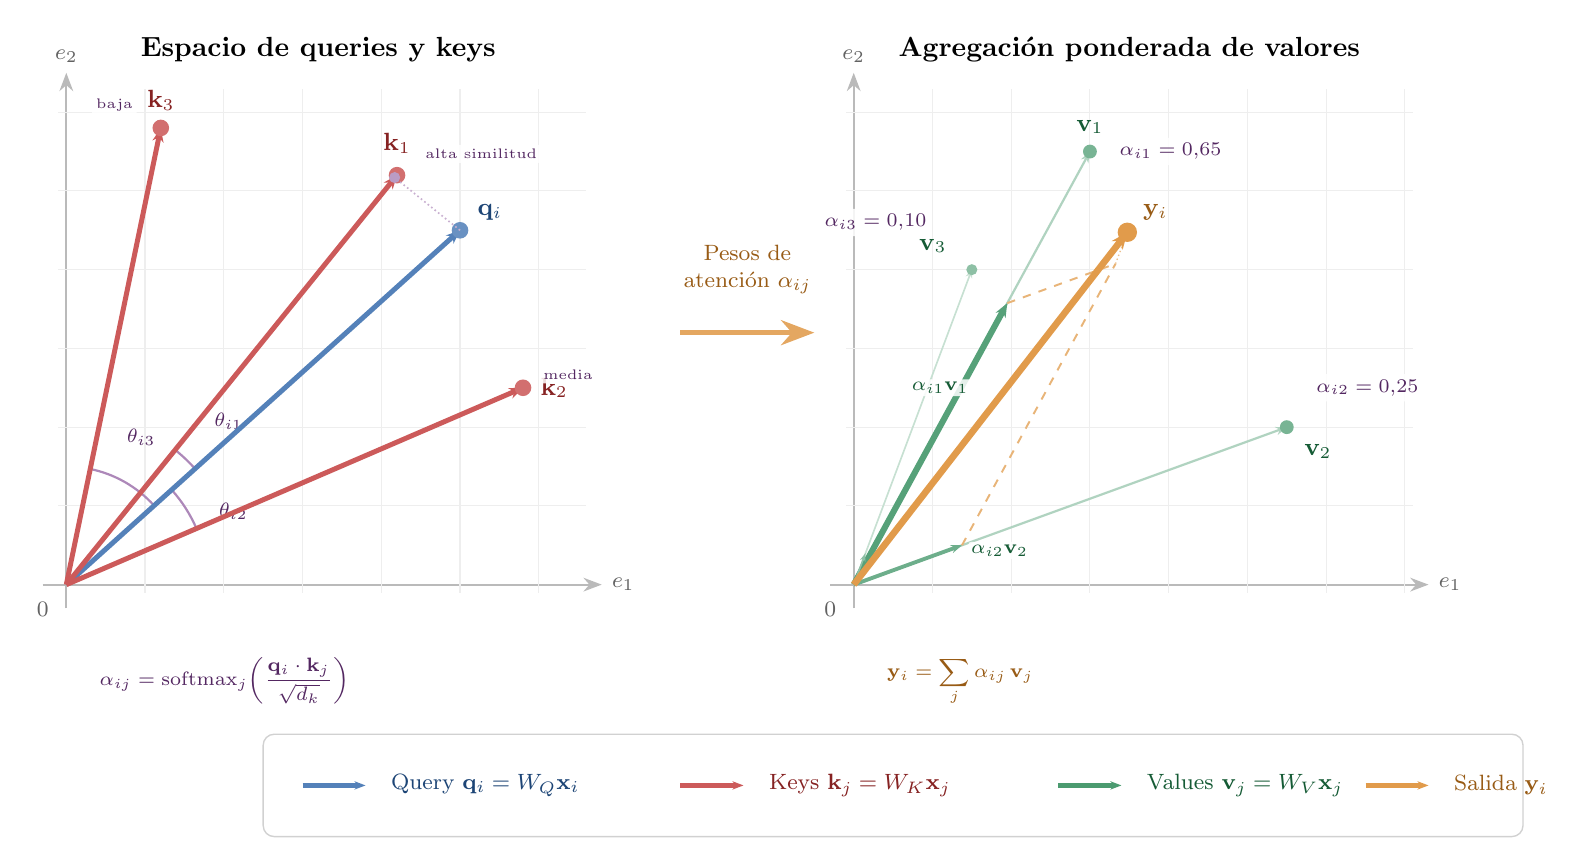
\begin{tikzpicture}[>=Stealth, font=\small]

% ============================================================
% LEFT PANEL: Query-Key space (dot-product similarity)
% ============================================================
\begin{scope}[shift={(0,0)}]

  % Title
  \node[font=\bfseries, align=center, text=black] at (3.2, 6.8)
    {Espacio de queries y keys};

  % Axes
  \draw[->, gdlgray!60, line width=0.8pt] (-0.3, 0) -- (6.8, 0)
    node[right, font=\footnotesize, text=gdlgray!70!black] {$e_1$};
  \draw[->, gdlgray!60, line width=0.8pt] (0, -0.3) -- (0, 6.5)
    node[above, font=\footnotesize, text=gdlgray!70!black] {$e_2$};

  % Light grid
  \foreach \x in {1,...,6} {
    \draw[gdlgray!15] (\x, -0.1) -- (\x, 6.3);
  }
  \foreach \y in {1,...,6} {
    \draw[gdlgray!15] (-0.1, \y) -- (6.6, \y);
  }

  % Origin label
  \node[font=\footnotesize, text=gdlgray!70!black, anchor=north east] at (-0.1, -0.1) {$0$};

  % === Angle arcs (draw BEFORE vectors so vectors overlay them) ===

  % Angles of vectors (degrees):
  %   q_i  = (5.0, 4.5)  -> atan2(4.5,5.0) = 41.99 ~ 42.0
  %   k_1  = (4.2, 5.2)  -> atan2(5.2,4.2) = 51.07 ~ 51.1
  %   k_2  = (5.8, 2.5)  -> atan2(2.5,5.8) = 23.33 ~ 23.3
  %   k_3  = (1.2, 5.8)  -> atan2(5.8,1.2) = 78.30 ~ 78.3

  % theta_{i1}: angle between q_i (42.0) and k_1 (51.1) -- small angle, high attention
  \draw[gdlpurple!60, line width=0.8pt]
    ({2.2*cos(42.0)}, {2.2*sin(42.0)}) arc[start angle=42.0, end angle=51.1, radius=2.2];
  \node[font=\scriptsize, text=gdlpurple!70!black, anchor=south west]
    at ({2.55*cos(46.5)}, {2.55*sin(46.5)}) {$\theta_{i1}$};

  % theta_{i2}: angle between k_2 (23.3) and q_i (42.0) -- moderate angle
  \draw[gdlpurple!60, line width=0.8pt]
    ({1.8*cos(23.3)}, {1.8*sin(23.3)}) arc[start angle=23.3, end angle=42.0, radius=1.8];
  \node[font=\scriptsize, text=gdlpurple!70!black, anchor=north west]
    at ({2.15*cos(32.5)}, {2.15*sin(32.5)}) {$\theta_{i2}$};

  % theta_{i3}: angle between q_i (42.0) and k_3 (78.3) -- large angle, low attention
  \draw[gdlpurple!60, line width=0.8pt]
    ({1.5*cos(42.0)}, {1.5*sin(42.0)}) arc[start angle=42.0, end angle=78.3, radius=1.5];
  \node[font=\scriptsize, text=gdlpurple!70!black, anchor=south]
    at ({1.9*cos(60)}, {1.9*sin(60)}) {$\theta_{i3}$};

  % === Query vector q_i ===
  \draw[-{Stealth[length=5pt,width=4pt]}, gdlblue!80, line width=1.8pt]
    (0,0) -- (5.0, 4.5);
  \node[font=\small, text=gdlblue!70!black, anchor=south west] at (5.1, 4.5)
    {$\mathbf{q}_i$};
  \fill[gdlblue!70] (5.0, 4.5) circle (3pt);

  % === Key vectors k_j ===
  % k_1: close to q_i (high similarity)
  \draw[-{Stealth[length=5pt,width=4pt]}, gdlred!80, line width=1.8pt]
    (0,0) -- (4.2, 5.2);
  \node[font=\small, text=gdlred!70!black, anchor=south] at (4.2, 5.35)
    {$\mathbf{k}_1$};
  \fill[gdlred!70] (4.2, 5.2) circle (3pt);

  % k_2: moderate similarity
  \draw[-{Stealth[length=5pt,width=4pt]}, gdlred!80, line width=1.8pt]
    (0,0) -- (5.8, 2.5);
  \node[font=\small, text=gdlred!70!black, anchor=west] at (5.9, 2.5)
    {$\mathbf{k}_2$};
  \fill[gdlred!70] (5.8, 2.5) circle (3pt);

  % k_3: low similarity (nearly orthogonal to q_i)
  \draw[-{Stealth[length=5pt,width=4pt]}, gdlred!80, line width=1.8pt]
    (0,0) -- (1.2, 5.8);
  \node[font=\small, text=gdlred!70!black, anchor=south] at (1.2, 5.9)
    {$\mathbf{k}_3$};
  \fill[gdlred!70] (1.2, 5.8) circle (3pt);

  % === Projection of q_i onto k_1 direction (illustrate dot product) ===
  % k1_hat = (4.2,5.2)/||(4.2,5.2)|| = (0.6280, 0.7781)
  % proj_len = 5*0.6280 + 4.5*0.7781 = 6.642
  % foot = 6.642*(0.6280,0.7781) = (4.171, 5.168) -- almost at k_1 tip
  \coordinate (projfoot) at (4.17, 5.17);
  \draw[gdlpurple!40, line width=0.6pt, densely dotted]
    (5.0, 4.5) -- (projfoot);
  \fill[gdlpurple!50] (projfoot) circle (2pt);

  % === Annotation: similarity labels next to each key ===
  \node[font=\tiny, text=gdlpurple!70!black, fill=white, fill opacity=0.85,
        text opacity=1, inner sep=1.5pt, rounded corners=1pt, anchor=south west]
    at (4.5, 5.35) {alta similitud};
  \node[font=\tiny, text=gdlpurple!70!black, fill=white, fill opacity=0.85,
        text opacity=1, inner sep=1.5pt, rounded corners=1pt, anchor=south west]
    at (6.0, 2.55) {media};
  \node[font=\tiny, text=gdlpurple!70!black, fill=white, fill opacity=0.85,
        text opacity=1, inner sep=1.5pt, rounded corners=1pt, anchor=south east]
    at (0.9, 5.95) {baja};

  % === Formula: dot product = similarity ===
  \node[font=\scriptsize, text=gdlpurple!70!black, align=center, anchor=north west]
    at (0.3, -0.8) {$\alpha_{ij} = \operatorname{softmax}_j\!\left(\dfrac{\mathbf{q}_i \cdot \mathbf{k}_j}{\sqrt{d_k}}\right)$};

\end{scope}

% ============================================================
% ARROW between panels
% ============================================================
\draw[->, gdlorange!70, line width=2pt] (7.8, 3.2) -- (9.5, 3.2);
\node[font=\footnotesize, align=center, text=gdlorange!70!black] at (8.65, 4.0)
  {Pesos de\\atenci\'{o}n $\alpha_{ij}$};

% ============================================================
% RIGHT PANEL: Weighted value aggregation
% ============================================================
\begin{scope}[shift={(10.0, 0)}]

  % Title
  \node[font=\bfseries, align=center, text=black] at (3.5, 6.8)
    {Agregaci\'{o}n ponderada de valores};

  % Axes
  \draw[->, gdlgray!60, line width=0.8pt] (-0.3, 0) -- (7.3, 0)
    node[right, font=\footnotesize, text=gdlgray!70!black] {$e_1$};
  \draw[->, gdlgray!60, line width=0.8pt] (0, -0.3) -- (0, 6.5)
    node[above, font=\footnotesize, text=gdlgray!70!black] {$e_2$};

  % Light grid
  \foreach \x in {1,...,7} {
    \draw[gdlgray!15] (\x, -0.1) -- (\x, 6.3);
  }
  \foreach \y in {1,...,6} {
    \draw[gdlgray!15] (-0.1, \y) -- (7.1, \y);
  }

  % Origin label
  \node[font=\footnotesize, text=gdlgray!70!black, anchor=north east] at (-0.1, -0.1) {$0$};

  % === Value vectors v_j (full, thin, as reference) ===

  % v_1: associated with k_1 (high attention alpha_{i1} = 0.65)
  \draw[-{Stealth[length=4pt,width=3pt]}, gdlgreen!35, line width=0.8pt]
    (0,0) -- (3.0, 5.5);
  \node[font=\small, text=gdlgreen!70!black, anchor=south] at (3.0, 5.6)
    {$\mathbf{v}_1$};
  \fill[gdlgreen!60] (3.0, 5.5) circle (2.5pt);

  % v_2: associated with k_2 (moderate attention alpha_{i2} = 0.25)
  \draw[-{Stealth[length=4pt,width=3pt]}, gdlgreen!35, line width=0.8pt]
    (0,0) -- (5.5, 2.0);
  \node[font=\small, text=gdlgreen!70!black, anchor=north west] at (5.6, 1.9)
    {$\mathbf{v}_2$};
  \fill[gdlgreen!60] (5.5, 2.0) circle (2.5pt);

  % v_3: associated with k_3 (low attention alpha_{i3} = 0.10)
  \draw[-{Stealth[length=3pt,width=2.5pt]}, gdlgreen!25, line width=0.6pt]
    (0,0) -- (1.5, 4.0);
  \node[font=\small, text=gdlgreen!70!black, anchor=east] at (1.3, 4.3)
    {$\mathbf{v}_3$};
  \fill[gdlgreen!50] (1.5, 4.0) circle (2pt);

  % === Weighted (scaled) value vectors -- shown as thick, prominent arrows ===

  % Coordinates:
  %   alpha_{i1} * v_1 = 0.65*(3.0, 5.5) = (1.95, 3.575)
  %   alpha_{i2} * v_2 = 0.25*(5.5, 2.0) = (1.375, 0.5)
  %   alpha_{i3} * v_3 = 0.10*(1.5, 4.0) = (0.15, 0.4)
  %   y_i = sum = (3.475, 4.475)

  % alpha_{i1} * v_1 (dominant contribution)
  \draw[-{Stealth[length=5pt,width=4pt]}, gdlgreen!75, line width=2.2pt]
    (0,0) -- (1.95, 3.575);
  \node[font=\scriptsize, text=gdlgreen!70!black, anchor=east,
        fill=white, fill opacity=0.85, text opacity=1, inner sep=1pt, rounded corners=1pt]
    at (1.5, 2.5) {$\alpha_{i1}\mathbf{v}_1$};

  % alpha_{i2} * v_2
  \draw[-{Stealth[length=4pt,width=3pt]}, gdlgreen!65, line width=1.4pt]
    (0,0) -- (1.375, 0.5);
  \node[font=\scriptsize, text=gdlgreen!70!black, anchor=north west,
        fill=white, fill opacity=0.85, text opacity=1, inner sep=1pt, rounded corners=1pt]
    at (1.45, 0.55) {$\alpha_{i2}\mathbf{v}_2$};

  % alpha_{i3} * v_3 (too small, show as tiny arrow)
  \draw[-{Stealth[length=3pt,width=2pt]}, gdlgreen!50, line width=0.6pt]
    (0,0) -- (0.15, 0.4);

  % === Parallelogram construction for vector addition ===
  % Step 1: alpha_{i1}*v_1 + alpha_{i2}*v_2 = (1.95+1.375, 3.575+0.5) = (3.325, 4.075)
  % Step 2: + alpha_{i3}*v_3 = (3.325+0.15, 4.075+0.4) = (3.475, 4.475)

  % Parallelogram: from tip of alpha_{i1}*v_1, translate by alpha_{i2}*v_2
  \draw[gdlorange!60, line width=0.7pt, dashed]
    (1.95, 3.575) -- (3.325, 4.075);
  % Parallelogram: from tip of alpha_{i2}*v_2, translate by alpha_{i1}*v_1
  \draw[gdlorange!60, line width=0.7pt, dashed]
    (1.375, 0.5) -- (3.325, 4.075);
  % Final small step: add alpha_{i3}*v_3
  \draw[gdlorange!50, line width=0.5pt, densely dotted]
    (3.325, 4.075) -- (3.475, 4.475);

  % === Output vector y_i ===
  \draw[-{Stealth[length=6pt,width=5pt]}, gdlorange!80, line width=2.4pt]
    (0,0) -- (3.475, 4.475);
  \node[font=\small\bfseries, text=gdlorange!70!black, anchor=south west] at (3.55, 4.5)
    {$\mathbf{y}_i$};
  \fill[gdlorange!80] (3.475, 4.475) circle (3.5pt);

  % === Weight annotations (placed away from vectors, near the reference v_j) ===
  \node[font=\scriptsize, text=gdlpurple!70!black, fill=white, fill opacity=0.85,
        text opacity=1, inner sep=2pt, rounded corners=1pt, anchor=west]
    at (3.3, 5.5) {$\alpha_{i1} = 0{,}65$};
  \node[font=\scriptsize, text=gdlpurple!70!black, fill=white, fill opacity=0.85,
        text opacity=1, inner sep=2pt, rounded corners=1pt, anchor=west]
    at (5.8, 2.5) {$\alpha_{i2} = 0{,}25$};
  \node[font=\scriptsize, text=gdlpurple!70!black, fill=white, fill opacity=0.85,
        text opacity=1, inner sep=2pt, rounded corners=1pt, anchor=east]
    at (1.0, 4.6) {$\alpha_{i3} = 0{,}10$};

  % === Output formula ===
  \node[font=\scriptsize, text=gdlorange!70!black, align=center, anchor=north west]
    at (0.3, -0.8) {$\mathbf{y}_i = \displaystyle\sum_{j} \alpha_{ij}\, \mathbf{v}_j$};

\end{scope}

% ============================================================
% LEGEND at the bottom
% ============================================================
\begin{scope}[shift={(3.0, -2.8)}]

  % Legend background
  \fill[white, rounded corners=4pt, draw=gdlgray!40, line width=0.5pt]
    (-0.5, -0.4) rectangle (15.5, 0.9);

  % Q entry
  \draw[-{Stealth[length=4pt,width=3pt]}, gdlblue!80, line width=1.6pt]
    (0, 0.25) -- (0.8, 0.25);
  \node[font=\footnotesize, text=gdlblue!70!black, anchor=west] at (1.0, 0.25)
    {Query $\mathbf{q}_i = W_Q \mathbf{x}_i$};

  % K entry
  \draw[-{Stealth[length=4pt,width=3pt]}, gdlred!80, line width=1.6pt]
    (4.8, 0.25) -- (5.6, 0.25);
  \node[font=\footnotesize, text=gdlred!70!black, anchor=west] at (5.8, 0.25)
    {Keys $\mathbf{k}_j = W_K \mathbf{x}_j$};

  % V entry
  \draw[-{Stealth[length=4pt,width=3pt]}, gdlgreen!80, line width=1.6pt]
    (9.6, 0.25) -- (10.4, 0.25);
  \node[font=\footnotesize, text=gdlgreen!70!black, anchor=west] at (10.6, 0.25)
    {Values $\mathbf{v}_j = W_V \mathbf{x}_j$};

  % Output entry
  \draw[-{Stealth[length=4pt,width=3pt]}, gdlorange!80, line width=1.6pt]
    (13.5, 0.25) -- (14.3, 0.25);
  \node[font=\footnotesize, text=gdlorange!70!black, anchor=west] at (14.5, 0.25)
    {Salida $\mathbf{y}_i$};

\end{scope}

\end{tikzpicture}
\end{document}
